% Failure analysis (hand-written; the cases were chosen by looking at report/figures/worst_te.png)
Most photos are segmented reasonably well (median object IoU on DUTS-TE \TeMedianIoU), but the distribution
has a long tail: \TeShareIoULow\% of DUTS-TE photos have object IoU below 0.1, which means the network picked
the wrong region entirely (Fig.~\ref{fig:iouhist}). Fig.~\ref{fig:failures} shows four such cases from DUTS-TE,
all with IoU 0.

\begin{figure}[H]
\centering
\IfFileExists{figures/iou_hist.png}{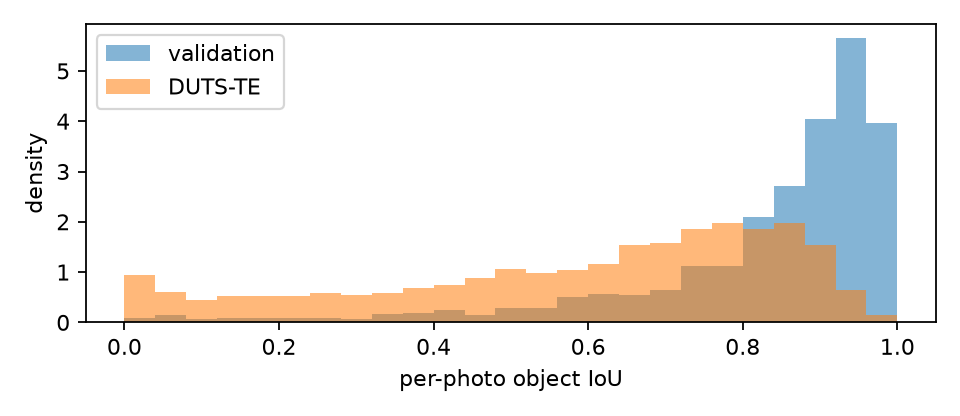
\includegraphics[width=0.62\linewidth]{figures/iou_hist.png}}{\fbox{pending}}
\caption{Per-photo object IoU on validation and DUTS-TE. DUTS-TE has many more near-zero failures.}
\label{fig:iouhist}
\end{figure}

\begin{figure}[H]
\centering
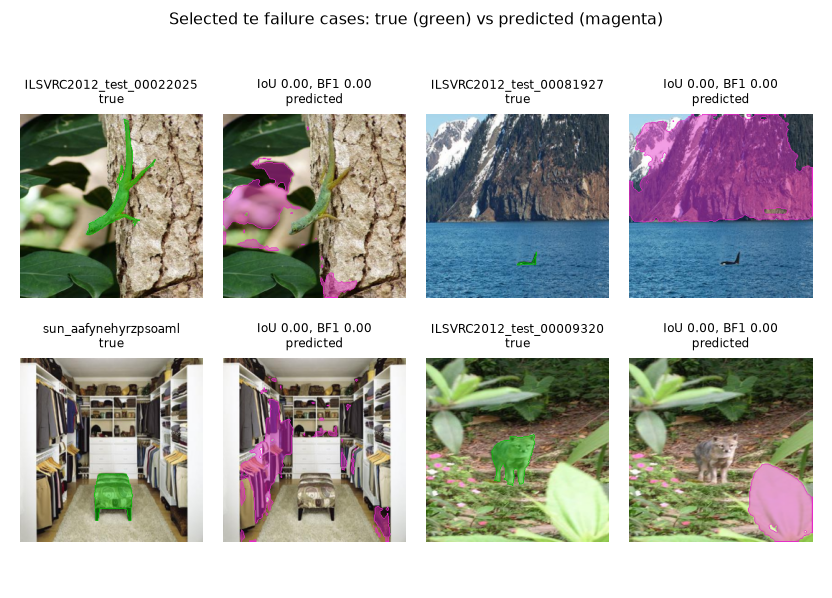
\includegraphics[width=0.92\linewidth]{figures/picked_te.png}
\caption{Four DUTS-TE failures (true mask green, prediction magenta).}
\label{fig:failures}
\end{figure}

\begin{enumerate}
  \item \textbf{Camouflage (lizard on bark, top left).} The green lizard has almost the same colour as the leaves and
        the same contrast as the bark texture. The network instead marks the large, blurred green leaf in the
        foreground. The lizard's thin legs and tail are 1--2 pixels wide at the network's $64\times64$ output, so
        even a correct detection would be hard to outline.
        \emph{Likely cause:} low colour and texture contrast between object and background, plus the coarse output.
  \item \textbf{Small, far object (orca, top right).} The orca covers well under 1\% of the photo, about 5 pixels
        across in the $128\times128$ input. The network segments the large, high-contrast mountain instead.
        \emph{Likely cause:} a small object. The global-context branch and the training data push the network
        towards large regions that stand out, and the low input resolution removes most of the small object's detail.
  \item \textbf{Clutter (walk-in closet, bottom left).} The annotated object is the ottoman in the centre, but the
        scene is full of clothes, shoes and shelves that are each just as distinctive. The network marks scattered
        pieces of the clothing and misses the ottoman, whose pattern blends with the rug.
        \emph{Likely cause:} a cluttered background with many candidate objects. Without enough context the network
        cannot tell which one the annotator meant.
  \item \textbf{Defocused foreground (kitten in plants, bottom right).} A large, bright, out-of-focus leaf at the
        bottom-right corner is predicted as the object, while the small grey kitten in the middle of the photo is
        missed. \emph{Likely cause:} a small, low-contrast object behind distracting foreground blur, which acts like
        partial occlusion.
\end{enumerate}

The validation failures (Fig.~\ref{fig:worstval}) show the same patterns: small objects (an insect on a tree trunk,
a bird on roof tiles) and camouflage (a scorpion lit in blue). They also show a further cause, \textbf{annotation
ambiguity}: in the savanna photo the ground truth marks the herd of zebras, but the lone tree is just as plausible
a ``main object'', and in the photo of a person holding a pretzel only the pretzel is marked. Such photos cap the
achievable score whatever the method.

\begin{figure}[H]
\centering
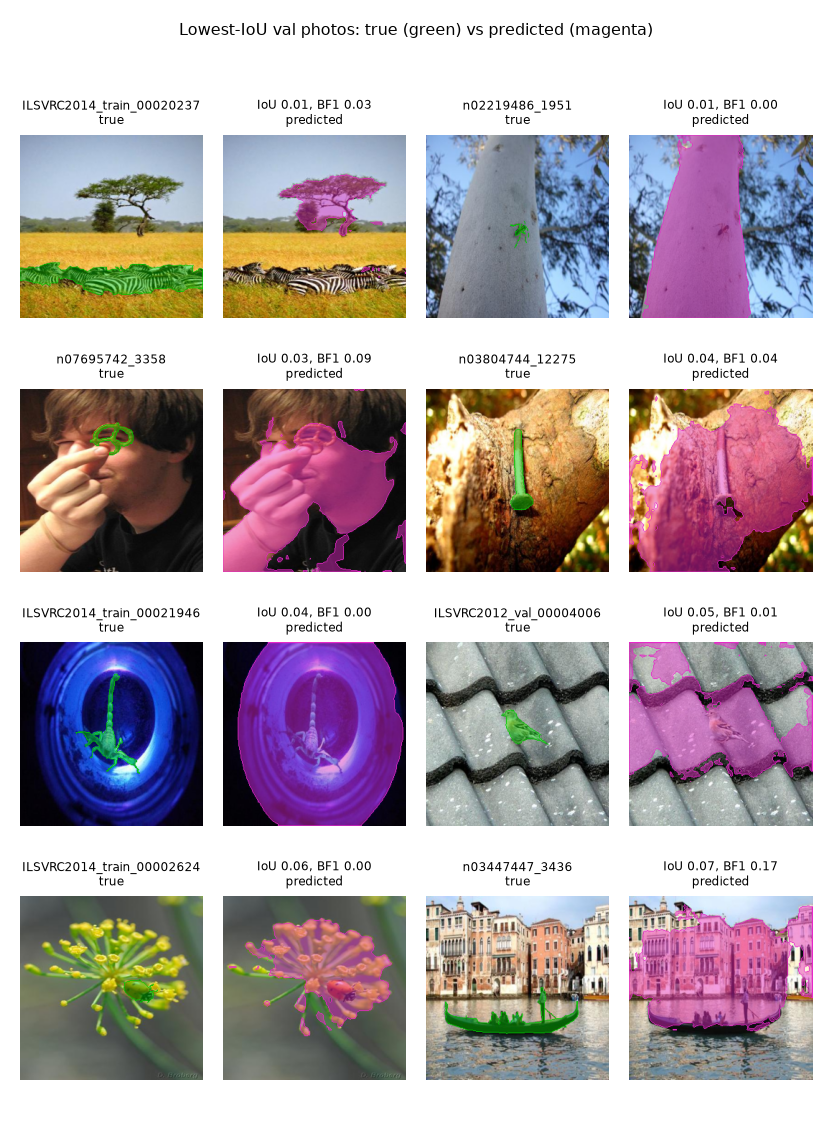
\includegraphics[width=0.85\linewidth]{figures/worst_val.png}
\caption{The eight lowest-IoU validation photos.}
\label{fig:worstval}
\end{figure}

These cases suggest specific fixes for my own training runs: zoom-out augmentation and a finer output (helping
small objects), a deeper or dilated context block (helping clutter), and colour and blur augmentation (helping
camouflage and defocus).
